\documentclass[tikz, border=3mm]{standalone}
\usepackage{tikz}
\usetikzlibrary{
    arrows.meta,         % For arrow tips
    decorations.markings,% For placing arrows along paths
    calc,                % For coordinate calculations
    positioning          % For label positioning
}

\begin{document}
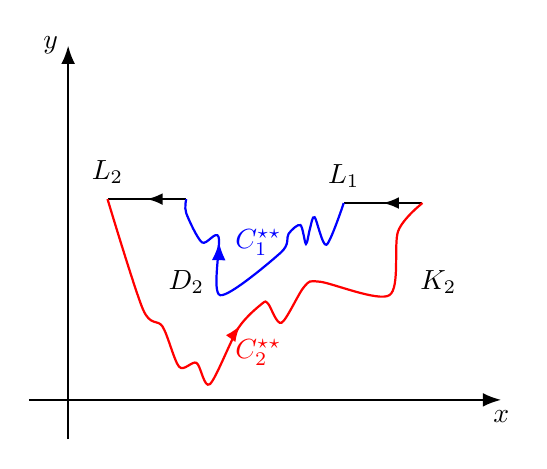
\begin{tikzpicture}[
    >=Latex, % Set default arrow tip style
    axis/.style={->, thick}, % Style for axes
    curve/.style={thick},    % Base style for curves
    line/.style={thick},     % Base style for lines
    cutstyle/.style={black, thick}, % Style for cut lines L1/L2
    % Style for placing an arrow in the middle of a path segment
    midarrow/.style={
        decoration={markings, mark=at position 0.5 with {\arrow{Latex[length=2mm]}}},
        postaction={decorate}
    },
     midarrowL/.style={
        decoration={markings, mark=at position 0.2 with {\arrowreversed{Latex}}},
        postaction={decorate}
    }
]

    % Axes
    \draw[axis] (-0.5, 0) -- (5.5, 0) node[below] {$x$};
    \draw[axis] (0, -0.5) -- (0, 4.5) node[left] {$y$};

    % Define coordinates for curve endpoints
    % Upper Cut Level
    \coordinate (A1) at (0.5, 2.55); % Start of Blue Curve / Left end of L2 Cut
    \coordinate (A)  at (1.5, 2.55); % Start of Red Curve / Right end of L2 Cut
    % Lower Cut Level
    \coordinate (B1) at (3.5, 2.5); % End of Blue Curve / Left end of L1 Cut
    \coordinate (B)  at (4.5, 2.5); % End of Red Curve / Right end of L1 Cut

    % Draw Horizontal "Cut" Lines L1 and L2
    \draw[cutstyle, midarrow] (A) -- (A1); % Line from A1 to A at y=1.5
    \node[above=2pt of A1] {$L_2$};

    \draw[cutstyle, midarrow] (B) -- (B1); % Line from B1 to B at y=0.5
    \node[above=2pt of B1] {$L_1$};

    % Draw Red Curve (from A to B)
    % Using Bezier curve with control points estimated from image
    % Controls pull curve above the horizontal lines
   % \draw[curve, red] (A1) .. controls (1.8, 2.2) and (0.95, 4.15) and (1.2, 2.93) and (1.41,2.42) and (1.63, 2.47) and (2.16, 2.91) and (2.46, 4.22) and (2.54, 4.22) and (2.71,3.98) and (3.0, 4.44) and (4.08, 3.33) and (4.19, 2.14) and (3.2, 1.5) .. (B);
    
    % Place arrow at position 0.5 (midway along path length)
            % Use \arrowreversed{>} to point against the path direction (clockwise)
    \draw [red, thick, midarrow] plot [smooth] coordinates {
   (0.5, 2.55)
   (0.95, 1.15)   
	(1.2, 0.93)
(1.41, 0.42)
(1.63, 0.47)
 (1.8, 0.2)
(2.16, 0.91)
(2.46, 1.22)
(2.54, 1.22)
(2.71, 0.98)
(3.0, 1.44)
(3.2, 1.5)
(4.08, 1.33)
(4.19, 2.14)
(4.5, 2.5)};

    % Draw Blue Curve (from A1 to B1)
    % Using Bezier curve with control points estimated from image
    % Controls keep curve between the horizontal lines
   % \draw[curve, blue] (A) .. controls (1.0, 1.0) and (2.0, 1.0) .. (B1);
    
    
    \draw [blue, thick, midarrowL] plot [smooth] coordinates {
    (1.5, 2.55)
    (1.5, 3.21-0.84)
(1.7, 2.7-0.7)
(1.91, 2.77-0.7)
(1.93, 3.23-1.9)
(2.7, 3.57-1.7)
(2.8, 2.81-0.7)
(2.95, 3.12-0.9)
(3.02, 2.68-0.7)
(3.07, 2.87-0.7)
(3.13, 3.02-0.7)
(3.28, 2.67-0.7)
(3.5,2.5)};

\node[black] (D2) at (1.5,1.5) {$D_2$};

\node[blue, right] (C1) at (2,2) {$C_1^{\star\star}$};

\node[red, right] (C2) at (2,0.6) {$C_2^{\star\star}$};

    % Optional: Add dots at the points if desired
    % \fill (A) circle (1.5pt);
    % \fill (B) circle (1.5pt);
    % \fill (A1) circle (1.5pt);
    % \fill (B1) circle (1.5pt);
    
        \node at (4.7, 1.5) {$K_2$}; % Position K1 to the right


\end{tikzpicture}
\end{document}